% this is the main file for each individual chapter
% each chapter has a subfolder, which contains a main.tex that simply inlines this file

\ifx\synctex\undefined\else\synctex=1\fi

\documentclass[b5paper,11pt]{book}

\usepackage[utf8]{inputenc}
%% (FMu) uzywamy \lw do napisania l z kreska, bo potem cos
%% przedefiniowuje \l na \lambda. To nie jest eleganckie,
%% ale dziala. To samo dla czeskiego hacka (np. w Cerny)
\let\lw\l  
\let\hacek\v

\usepackage{amsfonts}
\usepackage[fleqn]{amsmath} %fleqn does left alignment of display formulas
\usepackage{amssymb,amsmath}
\usepackage{amsthm}
\usepackage{graphicx}
\usepackage{xspace}
\usepackage{todonotes}
\usepackage{mathbbol}
\usepackage{enumerate}
\usepackage{comment}
\usepackage{enumitem}
\usepackage{hyperref}
\usepackage{bookmark}
\usepackage{nameref}
\usepackage{ifthen}
\usepackage{algorithm}
\usepackage[noend]{algpseudocode}
\usepackage{tikz}
\usepackage[normalem]{ulem}
\usepackage[all]{xy}
% \usepackage{mdframed} 
\usepackage{fancyhdr}
\usepackage{pdfpages}
\usepackage{mathtools}


\RequirePackage[osf,sc]{mathpazo}
\usepackage[mathcal]{euscript}



%style


\newcommand{\views}{\mathsf{views}}

\pagestyle{fancy}

\newcommand{\period}{.}%used in equations
\newcommand{\comma}{,}%used in equations

\newcommand{\tn}[1]{#1}% a number which is inlined in the text, and could be replaced by a word, e.g.
%has length at most \tn{3}
\newcommand{\an}[1]{$#1$}% a number which is inlined in the text, but represents an alphabet symbol,
%e.g. the set of words in which the number of \an{1}'s and \an{0}'s are equal.

%shrink bullets
\newlength{\mylen}
\newlength{\itemizemargin}%leftmargin for itemize lists
\newlength{\itemizelabelsep}%labelsep for itemize lists
\setbox1=\hbox{$\bullet$}\setbox2=\hbox{\tiny$\bullet$}
\setlength{\mylen}{\dimexpr0.5\ht1-0.5\ht2}
\setlength{\itemizemargin}{27pt}
\setlength{\itemizelabelsep}{\dimexpr 0.4\itemizemargin}
\renewcommand\labelitemi{\raisebox{\mylen}{\tiny$\bullet$}}
\renewcommand\labelitemii{\raisebox{\mylen}{\tiny$\bullet$}}
\setlist[itemize]{leftmargin=\itemizemargin,labelsep=\itemizelabelsep}

\newcommand{\tagsymbol}{$\diamond$}


\DeclareTextFontCommand{\textsmallcaps}{\scshape}

      \RequirePackage{letterspace}
      \RequirePackage{textcase}
      % Set up letterspacing (using microtype package) -- requires pdfTeX v1.40+
      \newcommand{\allcapsspacing}[1]{\textls[200]{#1}}
      \newcommand{\smallcapsspacing}[1]{\textls[50]{#1}}
      \newcommand{\allcaps}[1]{\textls[200]{\MakeTextUppercase{#1}}}
      \newcommand{\smallcaps}[1]{\smallcapsspacing{\scshape\MakeTextLowercase{#1}}}
      \renewcommand{\textsc}[1]{\smallcapsspacing{\textsmallcaps{#1}}}

\newcommand{\newlinetospace}[1]{#1}
% \DeclareRobustCommand{\newlinetospace}[1]{%
%   \let\@tufte@orig@cr\\% save the original meaning of \\
%   \def\\{\@tufte@newlinetospace}% turn \\ and \\* into \space
%   \let\newline\\% turn \newline into \space
%   #1%
%   \let\\\@tufte@orig@cr% revert to original meaning of \\
% }

\makeatletter
\newcommand*{\currentname}{\@currentlabelname}


\newcommand\iraggedright{%ragged right with indentation
  \let\\\@centercr\@rightskip\@flushglue \rightskip\@rightskip
  \leftskip\z@skip}



\newboolean{@test@}%if true, only parts encompassed in environment testshow will be typeset.
\setboolean{@test@}{true}

\newcommand{\testhide}[1]{
\ifthenelse{\boolean{@test@}}{}{#1}%in test mode contents is hidden
}


\newboolean{@tufte@symmetric}
\setboolean{@tufte@symmetric}{true}
\newboolean{@tufte@twoside}
\setboolean{@tufte@twoside}{true}


% The running heads/feet don't have rules
\renewcommand{\headrulewidth}{0pt}
\renewcommand{\footrulewidth}{0pt}
\newcommand{\plaintitle}{}
\newcommand{\plainauthor}{}
\setlength{\headsep}{45pt}
% The 'fancy' page style is the default style for all pages.
\fancyhf{} % clear header and footer fields
\newcommand{\headdisplay}[1]{{\fontsize{6.5}{0}\fontseries{b}\selectfont\scshape\textls[150]{#1}}}
\fancyhead[LE]{\thepage\quad\headdisplay{\leftmark}}%
\fancyhead[RO]{\headdisplay{\rightmark}\quad\thepage}


\renewcommand{\chaptermark}[1]%
   {\markboth{\MakeUppercase{#1}}{}}
\renewcommand{\sectionmark}[1]%
   {\markright{\MakeUppercase{#1}}}


\newlength{\@tufte@overhang}% used by the fullwidth environment and the running heads
\newlength{\@tufte@fullwidth}
\newlength{\@tufte@caption@fill}

\newcommand{\TufteRecalculate}{%
  \setlength{\@tufte@overhang}{\marginparwidth}
  \addtolength{\@tufte@overhang}{\marginparsep}

  \setlength{\@tufte@fullwidth}{\textwidth}
  \addtolength{\@tufte@fullwidth}{\marginparsep}
  \addtolength{\@tufte@fullwidth}{\marginparwidth}

  \setlength{\@tufte@caption@fill}{\textwidth}
  \addtolength{\@tufte@caption@fill}{\marginparsep}
}

\AtBeginDocument{\TufteRecalculate}
% Set the header/footer width to be the body text block plus the margin
% note area.
% \AtBeginDocument{%
%   \ifthenelse{\boolean{@tufte@symmetric}}
%     {\fancyhfoffset[LE,RO]{\@tufte@overhang}}
%     {\fancyhfoffset[RE,RO]{\@tufte@overhang}}
% }


\RequirePackage{titlesec,titletoc}
%%
% Make Tuftian-style section headings and TOC formatting

\titleformat{\part}%
  [display]% shape
  {\relax\ifthenelse{\NOT\boolean{@tufte@symmetric}}{\begin{fullwidth}}{}}% format applied to label+text
  {}%{\scshape \LARGE part\ \thepart\\}% label
  {0pt}% horizontal separation between label and title body
  {\Huge\rmfamily\itshape}% before the title body
  [\ifthenelse{\NOT\boolean{@tufte@symmetric}}{\end{fullwidth}}{}]% after the title body

\titleformat{\chapter}%
  [display]% shape
  {\relax\ifthenelse{\NOT\boolean{@tufte@symmetric}}{\begin{fullwidth}}{}}% format applied to label+text
  {\itshape\huge\thechapter}% label
  {0pt}% horizontal separation between label and title body
  {\huge\rmfamily\itshape}% before the title body
  [\ifthenelse{\NOT\boolean{@tufte@symmetric}}{\end{fullwidth}}{}]% after the title body


\titleformat{\section}%
  [hang]% shape
  {\normalfont\Large\itshape}% format applied to label+text
  {\normalfont\Large\itshape\thesection}% label
  {1em}% horizontal separation between label and title body
  {}% before the title body
  []% after the title body

\titlespacing*{\chapter}{0pt}{50pt}{40pt}
\titlespacing*{\section}{0pt}{3.5ex plus 1ex minus .2ex}{2.3ex plus .2ex}
\titlespacing*{\subsection}{0pt}{3.25ex plus 1ex minus .2ex}{1.5ex plus.2ex}


%%
% When \cleardoublepage is called, produce a blank (empty) page -- i.e.,
% without headers and footers
\def\cleardoublepage{\clearpage\if@twoside\ifodd\c@page\else
  \hbox{}
  %\vspace*{\fill}
  %\begin{center}
  %  This page intentionally contains only this sentence.
  %\end{center}
  %\vspace{\fill}
  \thispagestyle{empty}
  \newpage
  \if@twocolumn\hbox{}\newpage\fi\fi\fi}

%%
% Set the font sizes and baselines to match Tufte's books
\renewcommand\normalsize{%
   \@setfontsize\normalsize\@xpt{14}%
   \abovedisplayskip 10\p@ \@plus2\p@ \@minus5\p@
   \abovedisplayshortskip \z@ \@plus3\p@
   \belowdisplayshortskip 6\p@ \@plus3\p@ \@minus3\p@
   \belowdisplayskip \abovedisplayskip
   \let\@listi\@listI}
\normalbaselineskip=14pt
\normalsize
\renewcommand\small{%
   \@setfontsize\small\@ixpt{12}%
   \abovedisplayskip 8.5\p@ \@plus3\p@ \@minus4\p@
   \abovedisplayshortskip \z@ \@plus2\p@
   \belowdisplayshortskip 4\p@ \@plus2\p@ \@minus2\p@
   \def\@listi{\leftmargin\leftmargini
               \topsep 4\p@ \@plus2\p@ \@minus2\p@
               \parsep 2\p@ \@plus\p@ \@minus\p@
               \itemsep \parsep}%
   \belowdisplayskip \abovedisplayskip
}
\renewcommand\footnotesize{%
   \@setfontsize\footnotesize\@viiipt{10}%
   \abovedisplayskip 6\p@ \@plus2\p@ \@minus4\p@
   \abovedisplayshortskip \z@ \@plus\p@
   \belowdisplayshortskip 3\p@ \@plus\p@ \@minus2\p@
   \def\@listi{\leftmargin\leftmargini
               \topsep 3\p@ \@plus\p@ \@minus\p@
               \parsep 2\p@ \@plus\p@ \@minus\p@
               \itemsep \parsep}%
   \belowdisplayskip \abovedisplayskip
}
\renewcommand\scriptsize{\@setfontsize\scriptsize\@viipt\@viiipt}
\renewcommand\tiny{\@setfontsize\tiny\@vpt\@vipt}
\renewcommand\large{\@setfontsize\large\@xipt{15}}
\renewcommand\Large{\@setfontsize\Large\@xiipt{16}}
\renewcommand\LARGE{\@setfontsize\LARGE\@xivpt{18}}
\renewcommand\huge{\@setfontsize\huge\@xxpt{30}}
\renewcommand\Huge{\@setfontsize\Huge{24}{36}}

\makeatother


\renewcommand\qedsymbol{\scalebox{0.75}{$\blacksquare$}}

\fancypagestyle{plain}{
  \fancyhf{} % clear header and footer fields
  % Uncomment the following five lines of code if you want the opening page
  % of the chapter to express the folio in the lower outside corner.
  %\ifthenelse{\boolean{@tufte@twoside}}
  %  {\fancyfoot[LE,RO]{\thepage}}
  %  {\fancyfoot[RE,RO]{\thepage}}
}


  \titlecontents{part}%
    [3em] % distance from left margin
{\addvspace{3pt}\vspace{1.5\baselineskip}\LARGE\bfseries\itshape} % above (global formatting of entry)
    {\hspace*{0em}\contentslabel{2em}} % before w/label (label = ``2'')
    {\hspace*{0em}} % before w/o label
    {\rmfamily\upshape\qquad\thecontentspage} % filler + page (leaders and page num)
    [\vspace{5pt}] % after


  \titlecontents{chapter}%
    [3em] % distance from left margin
{\addvspace{3pt}\vspace{1.5\baselineskip}\LARGE\rmfamily\itshape} % above (global formatting of entry)
    {\hspace*{0em}\contentslabel{2em}} % before w/label (label = ``2'')
    {\hspace*{0em}} % before w/o label
    {\rmfamily\upshape\qquad\thecontentspage} % filler + page (leaders and page num)
    [\vspace{5pt}] % after

  \titlecontents{section}% FIXME
    [3em] % distance from left margin
    {\vspace{5pt}\vspace{0\baselineskip}\Large\rmfamily\itshape} % above (global formatting of entry)
    {\hspace*{2em}\contentslabel{2em}} % before w/label (label = ``2.6'')
    {\hspace*{2em}} % before w/o label
    {\rmfamily\upshape\qquad\thecontentspage} % filler + page (leaders and page num)
    [\addvspace{3pt}] % after

% (margin) notes 
%
\newcommand{\todonote}[2]{\todo[inline]{{\bf (#1)}: #2}}
\newcommand{\igw}[1]{\todo[size=\tiny,fancyline,color=blue!30]{{\bf (igw)}: #1}}
\newcommand{\ms}[1]{\todonote{MS}{#1}}
\newcommand{\sla}[1]{\todo[size=\tiny,fancyline,color=green!40]{{\bf (SL)}: #1}}
\newcommand{\slaInlini}[1]{\todonote{SL}{#1}}
\newcommand{\pawel}[1]{\todo[size=\tiny,fancyline,color=green!40]{{\bf (PP)}: #1}\xspace}
\newcommand{\henryk}[1]{\todo[size=\tiny,fancyline,color=orange!40]{{\bf (HM)}: #1}}
\newcommand{\sz}[1]{\todo[size=\tiny,fancyline,color=blue!40]{{\bf (sz)}: #1}}
\newcommand{\fmu}[1]{\todo[size=\tiny,fancyline,color=red!40]{{\bf (FMu)}: #1}}
\newcommand{\fma}[1]{\todo[size=\tiny,fancyline,color=purple!40]{{\bf (FMa)}: #1}}
\newcommand{\shu}[1]{\todo[size=\tiny,fancyline,color=green!40]{{\bf (SH)}: #1}}
\newcommand{\shuInlini}[1]{\todonote{SH}{#1}}
\newcommand{\eryx}[1]{\todo[size=\tiny,fancyline,color=green!40]{{\bf (EK)}: #1}}
%\newcommand{\wojtek}[1]{\todo[size=\tiny,fancyline,color=green!40]{{\bf (WC)}: #1}}
\newcommand{\wojtek}[1]{}

\newcommand{\mipi}[1]{\todo[size=\tiny,fancyline,color=blue!20]{{\bf (MiPi)}: #1}}
\newcommand{\klin}[1]{\todo[size=\tiny,fancyline,color=olive!20]{{\bf (BK)}: #1}}
\newcommand{\lorenzo}[1]{\todo[size=\tiny,fancyline,color=green!40]{{\bf (LC)}: #1}}
\newcommand{\joost}[1]{\todo[size=\tiny,fancyline,color=purple!40]{{\bf (JW)}: #1}}
\newcommand{\lorenzolong}[1]{\todonote{Wawrzyniec}{#1}}

% (SL) general
%
% star exercise
\newcommand{\starmark}{{\normalfont \upshape{\raisebox{0pt}{$(\ast)$}}}}
\newcommand{\starexercise}{\noindent \starmark\ }
% hint
\newcommand{\hint}[1]{\smallskip \noindent \smallcaps{Hint:}{\slshape\ #1}}
\newcommand{\note}{\smallskip \noindent \smallcaps{Note:}\ } %SH
% empty word
\newcommand{\emptyword}{\varepsilon}
% unified way of defining sets
\newcommand{\setof}[2]{\left\{#1 \,\mid\, #2 \right\}}
\newcommand{\set}[1]{\{#1\}}
% powerset
\newcommand{\powerset}[1]{{\cal P}(#1)}
% length of a word
\newcommand{\len}[1]{\lvert #1 \rvert}


\newcommand{\Nat}{\ensuremath{\mathbb{N}}}
\newcommand{\Int}{\ensuremath{\mathbb{Z}}}

\newcommand{\problemtitle}[1]{\smallcaps{#1}}
%some problems have titles, 
%which appear immediately at the beginning

%% math symbols

\newcommand{\unaryplus}{\raisebox{0.5pt}{\scalebox{0.65}{\( + \)}}}
\newcommand{\unaryminus}{\raisebox{0.5pt}{\scalebox{0.65}{\( - \)}}}
\newcommand{\cinc}{\unaryplus\unaryplus}%counter increment
\newcommand{\cdec}{\unaryminus\unaryminus}%counter decrement

%% math operators

\renewcommand\bar[1]{\overline{#1}}


% left composition symbol (Z notation)
%\DeclareMathSymbol{\fcmp}{\mathrel}{bbold}{\lq\;}
\newcommand{\fcmp}{\cdot}


% (SH)
\newcommand{\yesmark}{\checkmark}
\newcommand{\nomark}{\ensuremath{\times}\xspace}
% (SH)
\newcommand{\pairletter}[2]{\bigg[{{#1}\atop{#2}}\bigg]} 


%(Sz T) 
%uniformize set difference and inclusion
\renewcommand{\subset}{\subseteq}
\renewcommand{\setminus}{-}
% (FMu) disjoint union
\newcommand{\disunion}{+}

%the set of all infixes of a language L: \infixes L
\newcommand{\infixes}{\text{Infixes}}

%context-free grammar notation. Example: S\produce Sa \sep Sb \sep \emptyword
\newcommand{\produce}{\rightarrow}
\newcommand{\sep}{\mathop{\big|}}

%Pumping lemma notation: a long word in a context-free language decomposes as \prefix \pleft \infix \pright \suffix
\newcommand{\prefix}{\mathit{prefix}}
\newcommand{\infix}{\mathit{infix}}
\newcommand{\suffix}{\mathit{suffix}}
\newcommand{\pleft}{\mathit{left}}
\newcommand{\pright}{\mathit{right}}


\newcommand{\hatphi}{\widehat{\varphi}}
\newcommand{\hatgamma}{\widehat{\gamma}}

\newcommand{\leftpar}{\texttt{\upshape(}}
\newcommand{\rightpar}{\texttt{\upshape)}}
% (SL) Turing machines terminology
%
\newcommand{\initstate}{q_0}
\newcommand{\accstate}{q_f}
\newcommand{\blanksymb}{\textsc{b}}
\newcommand{\states}{Q}
\newcommand{\alphabet}{\Sigma}
\newcommand{\tapealphabet}{T}
\newcommand{\lewo}{\leftarrow}
\newcommand{\tutaj}{\circlearrowleft}
\newcommand{\prawo}{\rightarrow}
\newcommand{\transrules}{\delta}
% (SH)
\newcommand{\markend}{\$}

% (MS) ignore
\newcommand{\ignore}[1]{}

% (MS) Vertical letter with two coordinates
% i.e. \vletterab{a}{b} gives [a/b]
\newcommand{\vletterab}[2]{\left[\hspace{-5pt}\begin{array}{c} {#1} \\ {#2} \end{array}\hspace{-5pt}\right]}

% (MS) Vertical letter with three coordinates
% i.e. \vletterabc{a}{b}{c} gives [a/b/c]
\newcommand{\vletterabc}[3]{\left[\hspace{-5pt}\begin{array}{c} {#1} \\ {#2} \\ {#3} \end{array}\hspace{-5pt}\right]}

% (MS) A function
% i.e. \fun{f}{X}{Y} gives f : X -> Y
\newcommand{\fun}[3]{#1\colon #2 \to #3}

% (MS) A partial function
% i.e. \parfun{f}{X}{Y} gives f : X -' Y
\newcommand{\parfun}[3]{#1\colon #2 \rightharpoonup #3}

% (MS) A transition of an automaton
% i.e. p \tran{a} q
\newcommand{\tran}[1]{\xrightarrow{#1}}

% (MS) The equational symbol of definition
% i.e. L^n \eqdef L\cdot L \cdot\ldots \cdot L
%\newcommand{\eqdef}{\stackrel{\text{def}}=}

% (MS) The comprehension scheme symbol
% i.e. \{ w \mid w^2 \in L \}
\renewcommand{\mid}{:}

% (MS) The star in regular expressions
% i.e. w*\ast, \Sigma^\ast, L^\ast etc.
\renewcommand{\ast}{{*}}

% (MS) The plus in regular expressions
% i.e. w*\plus, \Sigma^\plus, L^\plus etc.
\newcommand{\plus}{{+}}

% (MS) The symbol used to reverse words and languages,
% i.e. L^\rev or w^\rev
\newcommand{\rev}{\mathrm{R}}

% (SH) operation of reversing
% i.e. \rev{L} or \rev{w}
\newcommand{\revop}[1]{{#1}^{\rev}}

% (MS) The operation constructing the cycled language:
% \cycle(L) = \{ uv : vu \in L \}
\newcommand{\cycle}{\mathrm{Cycle}\xspace}

% (FMu) The number of occurrences of word u in word w
% i.e. \occ{u,w}
\newcommand{\occ}[2]{\#_{#1}(#2)}


% (FMu) The automata font 
\newcommand{\aut}[1]{{\mathcal{#1}}}


% (MS) The set of non-trivial palindromes over a given alphabet
% i.e. \Pal_\Sigma = \{ u : u = u^\rev \wedge |u| \geq 2 \}
\newcommand{\Pal}{\mathrm{Pal}\xspace}

% (MS) The binary evaluation map \bin \colon \{0,1\}^* \to [0,1]
% i.e. \bin(101) = 0.625
\newcommand{\bin}{\mathrm{bin}\xspace}

% (WC)
% lowest common multiplicity
\newcommand{\lcm}{\mathrm{lcm}\xspace}
% label of the run
\newcommand{\lab}{\mathrm{lab}\xspace}
% size
\newcommand{\size}{\mathrm{size}}


%\renewcommand{\O}{\mathcal{O}}
\newcommand{\rank}{\mathit{rank}}
\newcommand{\floor}[1]{\lfloor #1 \rfloor}

\newcommand{\A}{\mathcal{A}}
\newcommand{\N}{\mathbb{N}}
\newcommand{\Z}{\mathbb Z}
\newcommand{\Q}{\mathbb Q}
\newcommand{\R}{\mathbb R}
\renewcommand{\P}{\mathbb P}
\newcommand{\E}{\mathbb E}
\newcommand{\F}{\mathcal F}
\newcommand{\G}{\mathcal G}
\renewcommand{\O}{\mathcal O}
\newcommand{\atoms}{\mathbb A}
\newcommand{\diff}{\textup{diff}}
\renewcommand{\inf}{\textup{inf}}
\newcommand{\xor}{\textup{inf-xor}}
\newcommand{\fxor}{\textup{fin-xor}}
\newcommand{\win}{\textup{Win}}
\newcommand{\attr}{\textup{attr}}
%\newcommand{\rank}{\textup{rank}}
\newcommand{\val}{\textup{val}}
%\newcommand{\len}{\textup{len}}
\newcommand{\first}{\textup{first}}
\newcommand{\last}{\textup{last}}
\newcommand{\nextpos}{\textup{next}}
\newcommand{\son}{\textup{son}}
\newcommand{\lson}{\textup{lson}}
\newcommand{\rson}{\textup{rson}}
\newcommand{\desc}{\textup{desc}}
\newcommand{\reach}{\textup{Reach}}
\newcommand{\tw}{\textup{tw}}
\newcommand{\minor}{\trianglelefteq}
\newcommand{\eso}{\exists\text{SO}}

% grammars terminology
%
% (SH) terminals (alphabet)
\newcommand{\terminals}{\Sigma} %TODO: dalem tak dla kompatybilnosci z tekstem Igora, ale mysle, ze powinno byc ujednolicone z \alphabet Slawka, czyli \newcommand{\terminals}{\alphabet}
% (SH) nonterminals (variables)
\newcommand{\nonterminals}{V}
% (SH) initial symbol
\newcommand{\initsymbol}{S}
% (SH) nonterminal associated with a terminal
\newcommand{\nontermletter}[1]{\fbox{$#1$}}
% (SH) nonterminal associated with a terminal that stores a state of a simulated automaton
%\newcommand{\nontermletterst}[2]{{#1}_{#2}}
% (SH) a leter with the word-end-marker
\newcommand{\letterend}[1]{#1^{\markend}}

\def\btrue{\textit{true}\xspace}
\def\bfalse{\textit{false}\xspace}
\renewcommand{\iff}{\Leftrightarrow}


% (MiPi) Complexity classes
\newcommand{\cmpclass}[1]{\smallcaps{#1}}
\newcommand{\cP}{\cmpclass{P}}
\newcommand{\cNP}{\cmpclass{NP}}
\newcommand{\cPSPACE}{\cmpclass{PSPACE\xspace}}
\newcommand{\cNPSPACE}{\cmpclass{NPSPACE\xspace}}
\newcommand{\cL}{\cmpclass{L}}
\newcommand{\cNL}{\cmpclass{NL}}

%TEXT
\newcommand{\leftmost}{left-most\xspace}
\newcommand{\rightmost}{right-most\xspace}

%%% FMu: quick and dirty aligning macro
\newcommand{\fantom}[1]{\textcolor{white}{#1}}

\newcommand{\zloty}{{\textsc{pln}}}
\newcommand{\euro}{{\textsc{eur}}}


%% Caligraphic

\newcommand{\Aa}{\mathcal{A}}
\newcommand{\Bb}{\mathcal{B}}
\newcommand{\Cc}{\mathcal{C}}
\newcommand{\Dd}{\mathcal{D}}
\newcommand{\Ee}{\mathcal{E}}
\newcommand{\Ff}{\mathcal{F}}
\newcommand{\Gg}{\mathcal{G}}
\newcommand{\Hh}{\mathcal{H}}
\newcommand{\Ii}{\mathcal{I}}
\newcommand{\Jj}{\mathcal{J}}
\newcommand{\Kk}{\mathcal{K}}
\newcommand{\Ll}{\mathcal{L}}
\newcommand{\Mm}{\mathcal{M}}
\newcommand{\Nn}{\mathcal{N}}
\newcommand{\Oo}{\mathcal{O}}
\newcommand{\Pp}{\mathcal{P}}
\newcommand{\Qq}{\mathcal{Q}}
\newcommand{\Rr}{\mathcal{R}}
\newcommand{\Ss}{\mathcal{S}}
\newcommand{\Tt}{\mathcal{T}}
\newcommand{\Uu}{\mathcal{U}}
\newcommand{\Vv}{\mathcal{V}}
\newcommand{\Ww}{\mathcal{W}}
\newcommand{\Xx}{\mathcal{X}}
\newcommand{\Yy}{\mathcal{Y}}
\newcommand{\Zz}{\mathcal{Z}}


\newcommand{\mypicf}[1]{
  \smallskip
	\begin{center}
		\includegraphics[page=#1,scale=0.25]{toolbox-figma}
	\end{center}
}


\newcommand{\mypic}[1]{
	\begin{center}
		\includegraphics[page=#1,scale=0.4]{pics}
	\end{center}
}

\newcommand{\mypicb}[1]{
	\begin{center}
		\includegraphics[page=#1,scale=0.4]{picsb}
	\end{center}
}

\newcommand{\mypicc}[1]{
	\begin{center}
		\includegraphics[page=#1,scale=0.4]{picsc}
	\end{center}
}

\newcommand{\namedpic}[2]{
$$
		\includegraphics[page=#1,scale=0.4]{picsb}  #2
$$
}


%% theorem environments for amsthm
%\theoremstyle{plain}
\newtheorem{theorem}{Theorem}[chapter]
\newtheorem{conjecture}[theorem]{Conjecture}
\newtheorem{lemma}[theorem]{Lemma}
\newtheorem{proposition}[theorem]{Proposition}
\newtheorem{corollary}[theorem]{Corollary}
\newtheorem{fact}[theorem]{Fact}
\newtheorem{claim}[theorem]{Claim}
\newtheorem{observation}[theorem]{Observation}
\newtheorem{sublemma}{Lemma}[theorem]
\newtheorem{definition}[theorem]{Definition}


\newcommand{\setbuild}[2]{\set{#1 \ | 
\begin{tabular}{l}
	#2
\end{tabular}}}

\newcommand{\myunderbrace}[2]{\underbrace{#1}_{\mathclap{\text{\scriptsize 
\begin{tabular}{c}
	#2
\end{tabular} }}}}

\newcounter{ourexamplecounter}
\newenvironment{example}{
\medskip

\refstepcounter{ourexamplecounter}
\smallskip\noindent{\textbf{{Example \arabic{ourexamplecounter}. }}}}{
$\Box$ \smallskip 
}

\DefineNamedColor{named}{IllustratorBlue}{cmyk}{0.6711,0.657,0,0}
\newcommand{\red}[1]{{\color{red}#1}}
\newcommand{\blue}[1]{{\color{IllustratorBlue}#1}}


\newcommand{\eqdef}{\stackrel{\text{def}} =}

\newcommand{\field}{\mathbb Q}

\newcommand{\sst}{{\sc sst}\xspace}
\newcommand{\mso}{{\sc mso}\xspace}
\newcommand{\nfa}{{\sc nfa}\xspace}
\newcommand{\dfa}{{\sc dfa}\xspace}

\newcommand{\Rat}{\mathbb Q}
\newcommand{\algebraic}{\bar{\mathbb Q}}
\newcommand{\gener}[1]{\langle #1 \rangle}
\newcommand{\aalg}{\mathbf A}
\newcommand{\balg}{\mathbf B}
\newcommand{\pol}[2]{\mathsf{pol}_{#1}{#2}}

\newcommand{\ratfun}{\mathsf{Rat}}
\newcommand{\seqfun}{\mathsf{Seq}^{\to}}
\newcommand{\seqfunrev}{\mathsf{Seq}^{\leftarrow}}
\newcommand{\sstfun}{\mathsf{SST}}
\newcommand{\twofun}{\mathsf{2Det}}
\newcommand{\regifun}{\mathsf{Regi}}

%%% Local Variables:
%%% mode: latex
%%% TeX-master: "EN_main"
%%% End:


\begin{document}
\frontmatter 

\thispagestyle{empty}

\mainmatter   % arabic page numbers
\pagestyle{fancy}

\renewcommand{\mypicf}[1]{
  \smallskip
	\begin{center}
		\includegraphics[page=#1,scale=0.25]{../toolbox-figma}
	\end{center}
}

\renewcommand{\mypic}[1]{
  \smallskip
	\begin{center}
		\includegraphics[page=#1,scale=0.25]{../pics}
	\end{center}
}

\renewcommand{\mypicb}[1]{
  \smallskip
	\begin{center}
		\includegraphics[page=#1,scale=0.25]{../picsb}
	\end{center}
}

\newcommand{\exercise}[3]{
    \paragraph*{Problem.} #1
    \paragraph*{Solution.} #3
}

In this chapter, we talk about transducers, i.e.~automata that input words and output words. We cover three families  of transducers as shown below:  \mypic{92}
\section{Sequential   functions}
Recall the definition of a \emph{nondeterministic finite automaton with output} from Definition~\ref{def:nfa-with-output}. This is an \nfa  where every transition is labelled by a  (possibly empty) \emph{output word} over a designated output alphabet, and every final state is labelled by a (possibly empty)  \emph{end-of-input word}, also over the output alphabet. Here is an example:
\mypic{114} 
 The output of a run is obtained by concatenating the output words of all transitions used, followed by the end-of-input word of the last state used. The semantics of the automaton is defined to be the function which maps an input word to the multiset of words over the output alphabet that are produced by accepting runs (if the same output is produced by $n$ different accepting runs, then it appears $n$ times in the output multiset).
 
  The automaton in the picture above has the following outputs: if the input word is empty, then the output multiset is empty; if the input word is nonempty, then the automaton produces exactly one output (i.e.~a multiset with one word) which is obtained from the input by deleting the first letter, doubling the other letters, and appending $b$ to the end.

 Define a \emph{\dfa with output} to be the special case of an \nfa with output where: (a) the transition relation is a deterministic, i.e.~for every state there is a unique outgoing transition for each input letter; and (b) all states are final. Under these assumptions, the automaton produces exactly one output for every input, and therefore its  semantics can be viewed as a function from words over the input alphabet to words over the output alphabet. Any function obtained this way is called  a \emph{(left-to-right) sequential function}\footnote{ The name sequential is used for  at least four transducer models in the literature, starting with the original transducer models described by Shannon~\cite[Section 8]{shannon1948mathematical} and later developed by  Moore~\cite{Moore:gu}
  and Mealy~\cite{Mealy:1955hu}. Both the Moore and Mealy models -- which are two non-equivalent models of letter-to-letter transducers -- were called sequential by their authors. In those days, sequential seems to have been a synonym for ``recognised by an automaton''. Then, Ginsburg introduced a model, called submachines, that could produce  words (and not just letters) in transitions~\cite{Ginsburg:1960ca}. Soon Ginsburg's model started to be called sequential, see e.g.~\cite[p.~298]{Eilenberg:1974vl}. Then,  Sch\"utzenberger extended submachines with end-of-input words~\cite{Schutzenberger:1977ck}. Now  it is Sch\"utzenberger's model -- originally called subsequential -- that is  being called sequential, e.g.~\cite{Filiot:2016iw}, and this is the convention that we adopt here.   }
.  Here is  an example: \mypic{46}
 The transducer above erases $a$'s at even-numbered positions, and appends $\#$ or nothing to the output, depending on the parity of the input length.
Other examples of  left-to-right sequential functions  include: ``erase all appearances of letter $a$'' or ``erase all appearances of letter $a$ at even-numbered input positions''.

  Define a \emph{right-to-left sequential function} symmetrically: the syntax is the same, except that in the semantics, the input letters are read from right to left, and the end-of-input word is produced after reading the leftmost position. The function ``identity if the input ends with $a$, otherwise empty output'' is a right-to-left sequential function but not a left-to-right sequential function.


 

\section{Rational functions} We now move to a richer class of functions from words to words, called the \emph{rational functions}\footnote{The name rational comes from Eilenberg. Eilenberg introduced rational subsets of any monoid~\cite[Chapter VII]{Eilenberg:1974vl}, which covers the special case of rational relations~\cite[Chapter IX]{Eilenberg:1974vl} defined  as rational subsets of monoids of the form~$\Sigma^* \times \Gamma^*$, which in turn covers the special case of \emph{rational functions} which are functional rational relations. }.  This class admits several equivalent definitions; we give five.  Another advantage is that the class is symmetric, i.e.~there is no need to define ``right-to-left rational functions''. We begin with two definitions that use \nfa's with output.

\paragraph*{Functional and unambiguous \nfa's with output.}
We say that  an  \nfa with output  is \emph{functional} if for every input word, the output multiset contains exactly one word, but possibly with multiplicities.  In other words,  there might be several accepting runs, but all accepting runs produce the same output word, and there is always at least one accepting run. 
We say that an \nfa with output  is \emph{unambiguous} if for every input word, the output multiset contains exactly one word, used exactly one time.   In other words, for every input there is exactly one accepting run. Functional, and therefore also unambiguous,  \nfa's with output can be viewed as recognising functions from words to words, by mapping an input word to the unique output word  in the output multiset. Functional \nfa's with output are essentially the same as the original definition of rational functions given by Eilenberg in~\cite[Chapter IX]{Eilenberg:1974vl}.

We will later show that -- when viewed as recognisers of functions from words to words (without multiplicities of outputs) --  functional and unambiguous automata have the same expressive power, i.e.~nothing is gained by using functional but possibly ambiguous \nfa's with output. 

%\begin{example}
%The following unambiguous \nfa with output realises the function "identity if the last letter is $a$, otherwise erase the entire word".
%\mypic{88}
%	\end{example}

\paragraph*{Lookahead \dfa with output.}
A \emph{lookahead \nfa with output} is a model that extends an \nfa with output as follows: instead of pairs (input letter, word over the output alphabet), the transitions are pairs (regular language over the input alphabet,  word over the output alphabet). A transition  labelled by a pair $(L,w)$ can be applied if the unread part of the input belongs to $L$; the effect of using such transition is that $w$ gets added to the output and one input letter is consumed. Here is a picture of a run:
\mypicc{52} 
 A \emph{lookahead \dfa with output} is the special case where (a)  for every state, the regular languages labelling outgoing transitions form a partition of all nonempty words; and (b) every state is final.


\begin{example}
The following lookahead \dfa with output swaps the first and last letters: \mypic{115}
\end{example}


\paragraph*{Eilenberg bimachine.} We now present Eilenberg bimachines, which are essentially another syntax for lookahead \dfa with output. An \emph{Eilenberg bimachine}~\cite[Chapter XI.7]{Eilenberg:1974vl} consists of two finite automata $\Aa, \Bb$ over the input alphabet -- with $\Aa$ left-to-right deterministic and $\Bb$  right-to-left  deterministic --  as well as an output function of type
\begin{align*}
\text{states of $\Aa$} \times \text{input alphabet} \times \text{states of $\Bb$} \quad \to \quad (\text{output alphabet})^*.
\end{align*}
In the automata $\Aa,\Bb$ the final states are irrelevant and can be omitted from the syntax.
The semantics of the bimachine is defined as follows. Given a nonempty input word,  define for each position in the input word an output word as described in the following picture: \mypicc{53}
The output of the bimachine is defined to be the concatenation of the output words, in the order inherited from the input positions.  To deal with empty inputs, an Eilenberg bimachine is equipped with an designated output word that is used for the empty input.


\paragraph*{Equivalence of the models.} The following theorem shows that all  the models described above are equivalent. We use the name \emph{rational function} for a word-to-word function that is defined by any one of the  equivalent models in the theorem. 
  \begin{theorem}\label{thm:rational-functions}
The following models are equivalent, in terms of the functions from words to words that they define:
\begin{enumerate}
	\item functional \nfa with output;
\item  lookahead \dfa with output;
 \item  unambiguous \nfa with output.
 \item  Eilenberg bimachines.
 \item compositions of right-to-left sequential functions with  left-to-right sequential functions.
\end{enumerate}	
\end{theorem}

\begin{proof}[Proof sketch.]\ 
\begin{itemize}
	\item[1 $\subseteq$ 2] Consider a functional \nfa with output $\Aa$. We define an equivalent  lookahead \dfa as follows. The lookahead \dfa computes some run of the functional \nfa that can be extended to an accepting run. Each transition is chosen using the lookahead, to determine if it can be extended to an accepting run.  If more than one transition can be chosen, some arbitrary tie-breaking mechanism is used.
\item[2 $\subseteq$ 3] Consider some  lookahead \dfa with output $\Aa$. We define an equivalent Eilenberg bimachine as follows.  Let $\Bb$ be a   right-to-left \dfa (without output) that simultaneously recognises all the languages which are used in the transitions of $\Aa$, i.e.~the lookahead languages. The simulating \nfa with output guesses the runs of these two automata (the run for $\Bb$ is right-to-left, and the run for $\Aa$ is left-to-right, and depends on the run of $\Bb$). This guess is unambiguous, because the automata $\Aa$ and $\Bb$ are unambiguous.
\item[3 $\subseteq$ 4] Consider an unambiguous \nfa with output $\Aa$. We define an equivalent  Eilenberg bimachine as follows.  The left-to-right automaton is a left-to-right powerset construction applied to states of $\Aa$, i.e.~its states are sets of states in $\Aa$ and the transition function is defined by
\begin{align*}
P \cdot a  = \set{ q : \text{the automaton $\Aa$ has a transition $p \stackrel {a/w} \to q
$ for some $p \in P$ }}	.
\end{align*}
The right-to-left automaton is defined symmetrically, i.e.~its transition function is defined by
\begin{align*}
a \cdot P   = \set{ p : \text{the automaton $\Aa$ has a transition $p \stackrel {a/w} \to q
$ for some $q  \in P$ }}	
\end{align*}
The output function maps a triple $(P,a,Q)$ to the unique output  word $w$ such that the automaton has a transition
\begin{align*}
p \stackrel {a/w} \to q \qquad p \in P, q \in Q.
\end{align*}
This function is well defined by the assumption that $\Aa$ is unambiguous.
\item[4 $\subseteq$ 1] Consider an Eilenberg bimachine $\Aa$. We define an equivalent functional  -- in fact, unambiguous -- \nfa with output as follows. The states of the simulating automaton are pairs (state of the left-to-right automaton in $\Aa$, state of the right-to-left automaton $\Aa$). The transition relation is defined by
\begin{align*}
(q,a p) \stackrel {a/w} \to (q a, p)	
\end{align*}
$w$ is the output word in the bimachine that is associated to the triple $(q,a,p)$. This automaton is unambiguous by the determinism assumptions in the definition of a bimachine.
\item[2 $\subseteq$ 5] A right-to-left sequential function can label the input word with states of right-to-left automata recognising the lookahead, and a left-to-right  sequential function can then simulate the \dfa with lookahead.
\item[5 $\subseteq$ 3] Functional \nfa with output are closed under compositions and  generalise both left-to-right and right-to-left sequential functions.
\end{itemize}	

\end{proof}



\section{Deterministic two-way transducers}
We now turn to the most powerful class of transducers discussed in this chapter, namely \emph{deterministic two-way transducers}. In the next chapter, we will present an equivalent one-way model, which uses registers to store parts of the output.

\begin{definition}
	A \emph{deterministic two-way transducer} consists of:
\begin{itemize}
	\item finite \emph{input and output alphabets} $\Sigma$ and $\Gamma$;
\item  a finite set of \emph{states} $Q$ with a distinguished \emph{initial} state;
\item a transition function
$$ \delta : Q \times (\Sigma \cup \set{\vdash,\dashv}) \to \set{\text{accept}} \cup (Q \times \set{\text{left, stay, right}} \times \Gamma^*)$$

\end{itemize}

\end{definition}
The semantics of the transducer are defined similarly to Turing machines. Actually, the model is equivalent to a Turing machine where there is one read-only input tape and one append-only output tape. The automaton begins in the following configuration:
\mypicc{54} 
(For two-way automata, the head is over a letter, as opposed to one-way automata, where the head is between letters.) At any given moment, the automaton applies its transition function to its current state and the symbol under the head. The result of the transition might be ``accept'', in which case the automaton ends its run, or a triple (state, direction, output word), in which case the new state is assumed, the head is moved in the direction, and the output word is  appended to the output. The output letters are used in chronological order, i.e. those which are output at the beginning of the run are at the beginning of the output, regardless of the position of the head when executing the transition. The run of the automaton might fail, either by moving out of the word (i.e. moving left on the left marker or moving right on the right marker), or by entering an infinite computation that never sees a final state; such failing runs do not produce any output, and therefore the semantics of the automaton is a partial function from $\Sigma^*$ to $\Gamma^*$. 

Typical things that can be done using a two-way transducer are duplication or reversing the input. 
The main result of this chapter is that deterministic two-way automata are closed under composition.

\begin{theorem}[\cite{Aho:1970is,Chytil:1977wh}]\label{thm:two-way-compose}
	Functions recognised by deterministic two-way transducers are closed under composition.
\end{theorem}
 For sequential and rational functions, closure under composition is done using a straightforward product construction. For two-way automata, the construction is much more challenging, since the automata begin composed might choose to move in different directions. 
 
The rest of this chapter is devoted to proving Theorem~\ref{thm:two-way-compose}.
We do it in two steps. First, we show in Lemma~\ref{thm:two-way-seq-comp} a weaker version -- namely that deterministic two-way automata are closed under pre-composition with rational functions.  Then we bootstrap the weaker version to get composition with deterministic two-way automata.

\paragraph*{Rational preprocessing.}  We begin by proving that deterministic two-way transducers can be pre-composed with rational functions.
A different perspective on this result is that deterministic two-way transducers would not become more expressive if  equipped with ``regular lookaround'', i.e.~transitions that depend not only on the letter under the head, but also on some regular properties of the words to the left and right of the head.

\begin{lemma}\label{thm:two-way-seq-comp} Deterministic two-way transducers are closed under pre-composition with rational functions. In symbols,
\begin{align*}
\underbrace{\twofun}_{\substack{\text{functions recognised by} \\ \text{deterministic two-way automata}}}  = \qquad  \twofun \qquad \circ  \underbrace{\ratfun}_{\text{rational functions}}\end{align*}
\end{lemma}
\begin{proof}
The left-to-right inclusion is immediate, because the identity is a rational function.
For the converse inclusion, recall the following characterisation 
\begin{align*}
\ratfun = \underbrace{\seqfun}_{\substack{\text{left-to-right}\\ \text{sequential functions}}} \circ \underbrace{\seqfunrev}_{\substack{\text{right-to-left}\\ \text{sequential functions}}}
\end{align*}
from Theorem~\ref{thm:rational-functions}. By the above, to prove the theorem it is enough to show  
	\begin{align*}
\twofun \supseteq \twofun \circ \seqfun \qquad \twofun \supseteq \twofun \circ \seqfunrev.
\end{align*}
By symmetry of two-way automata, it is enough to prove the first inclusion. Summing up, it suffices to show that if $f$ is left-to-right sequential  and $g$ is recognised by a deterministic two-way transducer, as in the following diagram,
\begin{align*}
 \xymatrix@C=4cm{\Sigma^* \ar[r]^{\text{left-to-right sequential $f$}} \ar[dr]_{f \circ g} & \Gamma^* \ar[d]^{\text{two-way $g$}} \\ & \Delta^*}
\end{align*}
then the composition $f \circ g$ is also recognised by a deterministic two-way automaton. The difficulty is the  machines for $f$ and $g$ have different types of movement. 

	The idea for the proof comes from Hopcroft and Ullman~\cite[Lemma 3]{Ullman:2013ip}. To simplify notation, we assume that $f$ is letter-to-letter, i.e.~each transition of the underlying \dfa with output produces exactly one output letter, and there are no end-of-input words.  The proof for the general case -- without  the letter-to-letter assumption -- can be easily inferred from the special case.
	
Suppose that the two-way automaton recognising $g$ is in state $p$ over  the $i$-th position of its input (which is the output of $f$), like in the following picture: 
	\mypic{87}
 	Then the simulating two-way  automaton for the composition $g \circ f$ has its head over the $i$-th position of the input word (which is the input of $f$), and knows the states $p$ and $q$ described in the picture above.
	The question is how to maintain this information, especially when the simulated two-way automaton $g$ wants to move its head to the left.
The key insight is to consider the graph which describes the states of $f$ and how they are updated by the transition function. This graph looks likes this:
\mypic{97}
The vertices of the graph are configurations of $f$, i.e. pairs (state of $f$, column between positions in the word), and the edges correspond to transitions of the automaton. Each edge is labelled by an output letter. We number the columns beginning with 1. Because $f$ is deterministic, the graph is a forest.

Define $q_i$ to be the state of $f$  in the $i$-th column, i.e. after reading the first $i-1$ letters of the input word. The simulating  two-way automaton  uses the state $q_{i}$ to get the $i$-th letter in the output $f(w)$. Suppose that the head of the simulating two-way automaton is over some position $i$ in the input word, and the state $q_{i}$ of the oracle is known, as indicated by a red circle in the following picture:
\mypic{98}

We show below how to maintain the state of $f$  when simulating  one transition of the two-way automaton $g$. If the transition of the two-way automaton $g$ does not move the head, or moves it to the right, there is no problem, since the transition function of $f$ can be simply applied to the known state $q_i$.

The issue is when the simulated two-way automaton $f$ wants to move the head to the left, and we need to compute the state $q_{i-1}$. 

Here is the solution. In terms of the forest in the pictures above, we want to determine the unique child of the red node which has the initial configuration in its subtree. To find this unique child, we do the following.
We start by moving the head one step to the left, which identifies all possible candidates for the predecessor configurations. Here is the picture, with the candidates being coloured yellow:  
\mypic{99} 


If there is only one yellow configuration, i.e. only one candidate for the predecessor, then we are done. The more interesting case is when there is more than one yellow configuration. In this case, we keep moving to the left, and use green to colour all descendants of the yellow configuration (and therefore of the red configuration as well). For each green configuration we remember which of the yellow configurations is its ancestor.  Two cases may happen. 

\begin{enumerate}
	\item We might reach a column where all green configurations are descendants of the same  yellow configuration, as in this picture: \mypic{100}





In this case, the unique yellow configuration is the one that we want to compute. The question is how to return to this unique configuration? The solution is this: suppose that we stopped in column $i$, i.e.~all green configurations in column $i$ are descendants of the same yellow configuration, but this is not true for column $i+1$. We store  in our memory the state of the unique yellow configuration that is the ancestor of all green configurations in column $i$. Then we start moving to the right, storing in each column that states reachable from the green configurations in column $i+1$. We stop when this set becomes a singleton -- this happens exactly when we reach the column with the red node. Then we can move one step to the left and use our stored yellow state to determine the predecessor configuration of the red one.
\item  The remaining case is when we reach the first column at the beginning of the input. Here we do the same trick to return to the red configuration, and we can keep in our state which branch of the subtree corresponds to the computation of the past oracle. 

\end{enumerate}


\end{proof}

\paragraph*{Closure under composition.} Using Lemma~\ref{thm:two-way-seq-comp} on pre-compositions with rational functions, we  complete the proof of Theorem~\ref{thm:two-way-compose} on composition closure  of deterministic two-way transducers. For our proof, it is more convenient to use a definition -- clearly equivalent in terms of expressive power -- of two-way transducers where the initial configuration is  (initial state, end of input marker $\dashv$). 

 Fix  two deterministic two-way transducers  
\begin{align*}
  \xymatrix{\Sigma^* \ar[r]^{\blue f} & \blue \Gamma^* \ar[r]^{\red g} & \red \Delta^*}.
\end{align*}
We use the following colour coding.
The  first  alphabet $\Sigma$  is written in black.  \blue{Blue} is used for the states and output alphabet  of  $\blue f$.  \red{Red} is for the states and output alphabet  of $\red g$.  Our goal is to give a deterministic two-way transducer which recognises the composition $\red g \circ \blue f$.

We begin with a naive construction that will not work. Take some input word $w \in \Sigma^*$, and consider the configuration graph of $\blue f$ on this input word, which looks like this:
\mypicc{28}
Vertices of the graph -- the blue dots -- are pairs (state, position in $w$ extended with end markers), and the edges correspond to transitions. The transitions are labelled by output words from the intermediate alphabet $\blue \Gamma$. We 
can represent the configuration graph as a labelling of the input word, with arrows stored in the positions where they originate, and the descriptions of the end markers stored in the adjacent input positions.

The natural construction for the composition $\red g \circ \blue f$ would be to have an automaton which stores a state of $\red g$ and a pointer to one of the letters from $\blue \Gamma$ that are in the  label of an edge in the configuration graph, as in the following picture:
\mypicc{71}
The problem with this construction is that a vertex in the configuration graph might have several incoming edges. For example, suppose that in the situation from the above picture, the automaton $\red g$ decides to move its head to the  left and change the state to~$\red p$. Then the automaton for the composition $\red g \circ \blue f$ would not know which of the following two choices should be made:
\mypicc{72}


The solution -- and also the reason why we use rational preprocessing from Lemma~\ref{thm:two-way-seq-comp} --  is to restrict the configuration graph of $\blue f$ to edges that are reachable from the initial configuration.

\begin{lemma}\label{lem:two-way-reachable}
The following function is rational. The input is  a configuration graph of $\blue f$, like this:
  \mypicc{55}
The output is the same graph, but only with those edges that are  reachable from the initial configuration, like this:
  \mypicc{30}
\end{lemma}
\begin{proof} 
We assume that a configuration graph is represented as word   where each letter represents the outgoing transitions from one column (i.e.~position in the input word with end markers). Here is a picture of a letter
\mypicc{50}
For this claim,  it is convenient to use an Eilenberg bimachine as the representation of rational transducers. Given a position $i$ in a configuration graph, the bimachine generates the following information:
\mypicc{51}
The information can be generated by deterministic automata, as required by the definition of an Eilenberg bimachine, using the standard conversion of two-way automata (without output) to one-way automata.  
Based on this information and the label of the position $i$, one can determine which states in position $i$ are reachable from the initial configuration. In its output, the bimachine only leaves edges that originate from reachable states. 
\end{proof}

By Lemma~\ref{thm:two-way-seq-comp}, deterministic two-way transducers are closed under rational preprocessing, and by Lemma~\ref{lem:two-way-reachable} a rational function can restrict a configuration graph to reachable configurations. Therefore, 
 in order to find a deterministic two-way transducer for the composition $\red g \circ \blue f$, it suffices to give a deterministic two-way transducer which inputs configuration graph of $\blue f$ restricted to reachable configurations, like this:
\mypicc{30}
and outputs the value of $\red g$ on the labelling of the unique path from the starting configuration  to the  accepting configuration. Since the blue nodes have indegree at most one, this can be done using the naive construction described before Lemma~\ref{lem:two-way-reachable}.





% !TEX root = ../main.tex


\exercise{zad:wqo-wqo}{
Show that the following conditions are equivalent for every quasi-order (a binary relation that is transitive and reflexive, but not necessarily anti-symmetric):
\begin{enumerate}
	\item  every infinite sequence contains an infinite subsequence that is  increasing (not necessarily strictly);
\item there are no infinite strictly decreasing sequences (i.e.~the quasi-order is well-founded) and no  infinite antichains (an antichain is  a set of pairwise incomparable elements);
\item every upward closed set is the upward closure of a finite set.
\end{enumerate}
A quasi-order that satisfies the above conditions is called a wqo.
}
{
	We prove the equivalences 1 $\Leftrightarrow$ 2 and 2 $\Leftrightarrow$ 3. The implications 1 $\Rightarrow$ 2 and 3 $\Rightarrow$ 2 are straightforward, so only prove the converses.
	\begin{itemize}
\item 2 $\Rightarrow$ 1. Take some infinite sequence of elements in the quasi-order. By the Ramsey Theorem, there is an infinite subsequence where either: (a) elements are strictly decreasing; (b) elements are pairwise incomparable; or (c) elements are (not necessarily strictly) increasing. Item 2 rules out cases (a) and (b), so we are left with case (c).
\item 2 $\Rightarrow$ 3. Take some upward closed set $U$, and consider the minimal elements. Because the quasi-order is well founded (by item 2), every element of $U$ is above some minimal element, and therefore $U$ is the upward closure of its minimal elements. If we take one minimal element for each equivalence class (i.e.~equivalence in the sense of both bigger and smaller), then we are left with an antichain, and this antichain is necessarily finite (by item 2).
	\end{itemize}
}


\exercise{zad:09-01}{
Which of the  following ordered sets are  wqo's?
\begin{enumerate}
  \item $\N^2$ with lexicographic order;
  \item $\{a, b\}^*$ with lexicographic order;
  \item $\N$ with divisibility order, i.e. $x$ smaller than $y$ if $x \ | \ y$;
  \item $\Sigma^*$ with prefix order;
  \item $\Sigma^*$ with infix order;
  \item line segments with an order: $[a,b]$ smaller than $[c,d]$ if $(b < c) \vee (a = c \wedge b \leq d)$;
  \item graphs with subgraph order (remove some edges and some vertices);
  \item trees with subtree order (remove some nodes, but keep the descendant ordering).
\end{enumerate}
}
{
Answers are the following.
\begin{enumerate}
  \item Yes. Any pair, which is dominating in Dickson's order is also dominating in lexicographic
  order. So by Dickson's lemma lexicographic order is also a wqo.
  \item No. An infinite descending sequence is of the form: $b, ab, aab, aaab, \ldots$.
  \item No. Prime numbers are an infinite antichain.
  \item No. An infinite descending sequence is of the form: $b, ab, aab, aaab, \ldots$.
  \item No. An infinite descending sequence is of the form: $bb, bab, baab, baaab, \ldots$.
  \item Yes. There is no infinite descending sequence, because sum $a+b$ is decreasing.
  There is also no infinite antichain. Assume there is one. Let $[a,b]$ be an element of it.
  Any $[c,d]$ in the antichain has to have $c \leq b$. So there are finitely many options for $c$,
  so some two segments in the antichain are of the form $[c,d_1]$ and $[c,d_2]$. However
  they have to be comparable, contradiction.
  \item No. Cycles $C_n$ for $n \geq 3$ are an infinite antichain. The same works also for induced subgraph order.
  \item No. An infinite antichain is formed by trees, which are paths of length $n$ such that both end vertices have
  additionally two neighbors (all together three neighbors). The same example works for induced subgraph
  order.
\end{enumerate}
}




\exercise{zad:09-08}{
Show that if $(X, \leq_X)$ and $(Y, \leq_Y)$ are both wqos then
also $(X \times Y, \leq)$ is wqo, where $(x, y) \leq (x', y') \iff x \leq_X x' \wedge y \leq_Y y'$.
}
{
Consider an infinite sequence of elements of $X \times Y$.
By the fact that $\leq_X$ is wqo there exists an infinite subsequence such that
first coordinates form an increasing subsequence. Then in that subsequence by the fact
that $\leq_Y$ is wqo there exists a dominating pair on second coordinates. This pair
is thus also a dominating pair in the order $\leq$.
}





\exercise{zad:09-02}{
Prove the Infinite Ramsey Theorem: in every infinite clique, with edges coloured on finitely many colours
there is an infinite monochromatic subgraph, i.e. subgraph such that all the edges in it are coloured by the same colour.
}
{
We sort vertices from left to right. First vertex has infinitely many outgoing edges, at least one color appears infinitely
many times. We choose such a color an leave only neighbors of this first vertex $v_1$ which have such colored edge
to $v_1$. Then we take $v_2$ (in the filtered sequence), there also exists a color such that $v_2$ has infinitely many
neighbors (to the right) with this color. We one more time filter vertices to the right of $v_2$
leaving only these which have appropriately colored edge with $v_2$.
In that way we also define $v_3, v_4, \ldots$. We always keep already defined vertices to the left untouched.
In that way we define $v_k$ for every $k \in \N$ so we have an infinite sequence of vertices $v_i$.
Every one has a distinguished color, so there exists a color in which there are infinitely many vertices.
They form a monochromatic clique.
}



\exercise{zad:09-03}{
Let $(X, \preceq)$ be a wqo. Show that there is no infinite growing sequence of upward-closed subsets $X$,
i.e. no sequence
\[
U_1 \subsetneq U_2 \subsetneq \ldots,
\]
s.t. for all $i \in \N$ set $U_i \subseteq X$ is upward-closed wrt. $\preceq$.
}
{
Assume towards contradiction that such an growing sequence exists.
Let $x_1 \in U_1$ and for $i > 1$ let $x_i \in U_i \setminus U_{i-1}$.
Because $\preceq$ is wqo there are some $i < j$ such that $x_i \preceq x_j$.
This means that $x_i \in U_i \subseteq U_{j-1}$ and by the fact that $U_{j-1}$ is upward-closed also $x_j \in U_{j-1}$.
Contradiction.
}


%mikolaj: w jakiej reprezentacji compute?
\exercise{zad:09-04}{
Show that given a  $d$-dimensional VAS and $s \in \N^d$, one can compute the  set of all configurations from which $s$ is coverable.
Hint: use Problem~\ref{zad:09-03}.
}
{

}






\exercise{zad:09-05}{
Show that given a vector addition system with a distinguished source configuration, one can decide if the set of configurations reachable from the source is finite.
}
{
We build a tree with root being vector $s$ and children of every vector $v$ being all
the $v+t$ for $t \in T$ such that $v+t \in \N^d$. However we can this tree in the following way.
If there is some vertex $v \in \N^d$ such that there exists its ancestor vertex $u \in \N^d$ with $u \preceq v$ then we do not
continue expanding vertex $v$. There are two cases. If $v$ is strictly bigger than $u$ on some coordinate by detecting dominating
pair $(u, v)$ on this path we know that reachability set is infinite. In the other case, if $u = v$, we know that it makes no sense
to expand this path, because we will not reach anything new. By Dickson's lemma we know that every path is finite.
Tree is finitely branching, therefore by K{\"{o}}nigs lemma the whole tree is finite. Therefore at some moment
we will compute the whole tree an algorithm will be finished. If all dominating pairs where $u = v$ then reachability set
is finite, otherwise it is infinite.
}






\exercise{zad:wqo-higman}{
Prove the following version of Higman's Lemma: if $\Sigma$ is a finite alphabet, then $\Sigma^*$ ordered by (not necessarily connected) subword is a wqo.}
{
}

\exercise{zad:wqo-lossy}{
Define a \emph{rewriting system} over an alphabet $\Sigma$ to be finite set of pairs $w \to v$ where $w,v \in \Sigma^*$. Define $\to^*$ to be the least binary relation on  $\Sigma^*$ which contains $\to$, is transitive,  and satisfies
\begin{align*}
  w \to^* v \qquad \text{implies} \qquad aw \to^* av \text{ and } wa \to^* va \qquad \text{for every }a \in \Sigma.
\end{align*}
There exist rewriting systems where $\to^*$ is an undecidable relation. Show that $\to^*$ is decidable if the rewriting system is \emph{lossy} in the following sense: for every letter $a \in \Sigma$, the rewriting system contains  $a \to \varepsilon$.}
{
}

\exercise{zad:wqo-zvass}{Define a \emph{$\Int$-vector addition system} in the same way as a vector addition system, except that configurations are vectors in $\Int^d$.  Show that the reachability problem is decidable, i.e.~one can decide if there is a run connecting two given configurations.}
{
}


\exercise{zad:vass}{Define a \emph{vector addition system with states} to be a finite set of states $Q$, a dimension $d$, and a finite set $\delta \subseteq Q \times \Int^d \times Q$. A configuration is an element of $Q \times \Nat^d$, and a transition is a pair 
\begin{align*}
(q,x) \to (p,y)	 \qquad \text{such that }(q,y-x,p) \in \delta.
\end{align*}
Show that the following problem is decidable: given states $p,q$ decide if there is a run from the configuration $(p,\bar 0)$  to some configuration with state $q$.
}
{
}


\exercise{zad:wqo-vass-exponential}{
\wojtek{Moze lepiej zrobic zadanie o zbiorze osiagalnosci przy ustalonym poczatku, a nie relacji osiagalnosci?
Latwiej sie mysli wg mnie.}
Find a vector addition system, say of dimension $d$, where the reachability relation
\begin{align*}
\set{(x,y) : \text{there is a run from from $x$ to $y$}} \subseteq \Nat^{2d}
\end{align*}
is not semilinear. Hint: use states and try to simulate exponentiation.
}
{
}

%mikolaj: czy dimension ma byc fixed czy nie?
\exercise{zad:wqo-vass-reach}{
Find a family of  vector addition systems with states, say of dimension $d$ (the dimension does not need to be fixed for the family), where the reachability set
\begin{align*}
\set{v : \text{there is a run from from the origin to $v$}} \subseteq \Nat^{d}
\end{align*}
is finite, but
\begin{enumerate}
  \item of doubly exponential size,
  \item of tower size
\end{enumerate}
with respect to the number of transitions.}
{
}


\newpage
{\Huge \it Bibliography}

\bigskip
\renewcommand{\chapter}[2]{}
\bibliographystyle{plain}
\bibliography{bib}


\end{document}
